\chapter{Konzeption}
\label{ch:concept}

In diesem Kapitel werden die Schritte und Entscheidungen erläutert, die zur Erhebung der Daten und zum Training des Klassifizierers notwendig sind.
Dazu werden vorab einige Entscheidungen und Anforderung an die zu entwickelnden Module geknüpft.
Der Prozess von der Idee bis zur fertigen Inbetriebnahme schließt folgende vier Schritte ein, die in dieser Reihenfolge abgeschlossen werden müssen:

\begin{description}
    \item[Data Engineering] Die Daten müssen erhoben und mit dem Deep-Learning-Modell in Einklang gebracht werden.
    Aus rohen Videos und strukturierten \gls{annotationen} werden Samples in ein einheitliches \gls{ml}-Datenset überführt.
    \item[Training] Es muss ein einheitlicher Trainingsablauf definiert werden, um die Ergebnisse einzelner Experimente vergleichen zu können.
    Dabei werden Metriken zur Evaluation der Modelle erhoben.
    \item[Verifikation] Mithilfe des trainierten Klassifizierers wird ein Teil der Samples manuell verifiziert.
    Die Annotationen, auf denen die Samples basieren, können im Falle eines Datenfehlers manuell angepasst werden, um die Datenqualität zu verbessern.
    \item[Inferenz] Das trainierte Modell muss in eine zeitliche Action Detection integriert werden, sodass ungeschnittene Videos ganzer Spiele verarbeitet werden können.
    Schließlich muss der Klassifizierer in eine Nutzerschnittstelle integriert und bereitgestellt werden.
    Die Integration soll technisch ermöglicht werden, ist allerdings nicht mehr Bestandteil dieser Arbeit.
\end{description}

\section{Datenquellen und Datenformat}
\label{sec:datenquellen}

Essenziell für das Data-Engineering ist, dass die Trainingsdaten die richtigen Informationen enthalten, die es dem Modell erst ermöglichen notwendige Zusammenhänge zu abstrahieren.
Die Daten müssen genug Informationen enthalten, um die Spielaktion lernbar zu machen.
Zudem sollten die Daten ein möglichst diverses Spektrum und einen geringen Bias aufweisen und keine Ausrichtung auf spezielle Eigenschaften haben ~\cite{Gugger20}.
Aus den genannten Gründen wird sich dagegen entschieden nur Aufnahmen einer taktischen Kamera oder eines bestimmten Stadions zu verwenden.
Damit das \gls{har}-Modell ausreichend gut adaptiert werden kann, wird stattdessen der Versuch unternommen ein Datenset zu generieren, das Spiele verschiedener Mannschaften, Nationalitäten und Geschlechter beinhaltet.
Zudem soll das Videomaterial verschiedenen (TV-)Quellen zugrunde liegen, sodass sich das Modell nicht auf bestimmte Eigenschaften des Kameraschnitts (wie Art der Kameraführung, Wiederholungen, Einblendungen, Bildqualität) einschießt.

Um ein eigenes, ausreichend großes Datenset zu erstellen, werden in dieser Arbeit mehrere Datenquellen kombiniert und in ein einheitliches Dateiformat überführt.
Dabei wird die Erhebung von Videomaterial $X$ und die Erhebung von Aktionsannotationen $Y$ separat betrachtet.

\subsection{Aktionsannotationen}
\label{subsec:aktionsannotationen}

Da Videomaterial von Fußballspielen durch öffentliche oder kommerzielle Video-Plattformen im Internet vergleichsweise einfach zu finden ist, liegt der Fokus bei der Generierung des Datensets primär auf dem Beziehen akkurater Annotationen.
Die \gls{annotationen} müssen eine genaue zeitliche Auflösung haben, die mindestens im Sekundenbereich liegt.
Das liegt zum einen daran, dass Aktionen bei einem schnellen Spiel oft dicht aufeinander folgen und zum anderen daran, dass sich die Spielaktionen selbst nur wenige Sekunden lang sind.
Zusätzlich sollen Sie mehr Klassen als die bisherigen Datensets (SoccerNet und SoccerDB) einschließen.
Darüber hinaus unterliegt die Auswahl zusätzlicher Klassen einiger selbstauferlegter Kriterien:

\begin{description}
    \item[Visuelle Erkennbarkeit] Eine Aktion muss allein auf Basis visueller Reize innerhalb weniger Frames erkennbar sein.
    \item[Mindestanzahl an Beispielen] Aktionen müssen mit einer Mindestanzahl an \gls{annotationen} repräsentiert sein, damit sie in neuartigen Situationen sicher wiedererkannt werden können.
    Die untere Grenze wird bei 50 Beispielen festgesetzt.
    \item[Maximalanzahl an Beispielen] Einige Aktionen wie Pässe und Ballannahmen sind im Verhältnis zu anderen Aktionen so überrepräsentiert, dass sich praktische jeder dieser Aktionen mit mindestens einer weiteren Aktion zeitlich überlagert.
    Zudem erschwert es die abschließende zeitliche Action Detection, wenn mehrere gleiche Aktionen direkt hintereinander stattfinden:
    Wird \zB ein direkter Pass gespielt, erfolgt die Ballannahme gleichzeitig mit der Ballabgabe und es gibt keinen zeitlichen Puffer zwischen beiden Pass-Aktionen.
    Die hier verwendete Methodik kann solche Abfolgen von direkt folgender gleicher Aktionen also gar nicht auseinander halten und müsste sie als eine lange Aktion behandeln.
    \item[Objektive Regeln] Die Aktionen müssen durch ein eindeutiges Regelwerk definiert sein.
\end{description}

Als ein geeigneter Provider für \gls{annotationen} wird an dieser Stelle auf \gls{sbod}\footnote{Da die Sammlung kontinuierlich erweitert wird, bezieht sich die Bezeichnung \gls{sbod} im Folgenden auf den Stand vom 16.07.2020}~\cite{Statsbomb20} zurückgegriffen.
Dabei handelt es sich um eine frei nutzbare Sammlung professioneller \gls{annotationen} eines kommerziellen Anbieters.
Die Sammlung umfasst mehr als 28 Millionen detaillierte \gls{annotationen} aus 33 Oberkategorien (siehe~\cite{StatsbombDocs16}) zu 799 Spielen.
Die Spiele wurden zwischen 2003 und 2020 ausgetragen und beziehen sich auf zehn internationale Ligen -- davon drei aus dem Frauenfußball.
Jede der Oberkategorien hat teils zahlreiche zusätzliche Attribute, wodurch sich weitere Unterkategorien ableiten lassen.

In \gls{sbod} ist die Dauer einer Aktion, die mit einem Schuss oder Pass zusammenhängt definiert durch die Dauer, die der Ball zwischen Abspiel und Annahme (\bzw dem Rollen ins Aus oder ins Tor) zurücklegt.
Andere Aktionen, wie Tore oder Auswechslungen, sind (wie auch in SoccerNet) als Zeitpunkte definiert.
Damit alle Klassen in gleicher Weise durch Zeitintervalle repräsentiert werden können, werden angepasste Zeitfenster generiert.
So ein Zeitfenster ergibt sich aus einer Mindestdauer von zwei Sekunden, die um den besagten Zeitpunkt oder Mittelpunkt des Zeitintervalls aufgespannt wird.
Ist das Original-Zeitintervall größer als die Mindestdauer, bleibt es unverändert und wird so übernommen.

\subsection{Videomaterial}
\label{subsec:videomaterial}

Als erste Video-Datenquelle wird das öffentliche Datenset SoccerNet verwendet.
Die Videos zu den Spielen sind pro Halbzeit zugeschnitten und können separat heruntergeladen werden.
Die Spiele decken fünf europäische Ligen, sowie Spiele der UEFA Championsleague ab, die zwischen 2014 und 2017 ausgetragen wurden.
Die Videoqualität ist durchweg gut und liegt bei einer Auflösung von mindestens 720p (siehe~\cite{SoccerNet20}).
SoccerNet besteht neben 6,637 \gls{annotationen} aus 1,000 Videos von 500 Fußballspielen, wovon sich 41 mit den Spielen aus \gls{sbod} überschneiden.
Diese Menge wird im Vergleich zu anderen Datensets allerdings noch als deutlich zu klein eingeordnet (vgl. \autoref{tab:dataset}).

Daher wird der Großteil der Videos über öffentliche Kanäle der Video-Plattform YouTube bezogen.
Diese Videos sind nicht pro Halbzeit zugeschnitten und potenziell fehlerbehaftet (\zB durch herausgeschnittene Spielminuten oder eine abweichende Abspielgeschwindigkeit), was ein zusätzliches Pre-Processing erfordert (siehe \autoref{ch:data}).

\subsection{Speicherformat}
\label{subsec:zielformat}

Die Rohdaten aller oben genannten Quellen werden anschließend in ein Zielformat überführt.
Dazu findet vorab ein Matching statt, das jeweils Videos und Annotation für ein Spiel zusammenbringt.
Die erfolgreich gematchten Datensätze, werden in einer Datei persistiert, die Annotationen und Videos in Verbindung setzt.
\gls{har}-Datensets in der Regel nicht direkt als fertige Samples $(x_i, y_i)$ veröffentlicht, da die Input-Matrizen $x_i$ unkomprimiert sehr viel Speicher belegen.
Stattdessen werden die Daten in einem Zwischenformat (\zB CSV- oder JSON-Datei) gespeichert.
Diese strukturierten Dateien speichern jeweils Tupel aus einem Label, dem Verweis auf eine Videoquelle (als Link oder Dateiname), sowie Start- und Endmarkierungen, die angeben wann die Aktion im Video zu sehen ist.
Die rohen Videodaten sind also nicht direkter Bestandteil des Datensets, sondern müssen zur Laufzeit nachgeladen werden.
Als Speicherformat wird im Kontext dieser Arbeit \gls{json} gewählt, da es flexibel und hierarchisch angeordnet werden kann und damit vergleichsweise kompakt ist.

\section{Anwendbarkeit von HAR-Modellen}
\label{sec:decisions}

Neben der passenden Datengrundlage werden im nächsten Schritt geeignete \gls{har}-Modelle und zu optimierenden Hyperparameter ausgewählt.
Anforderungen an ein passendes \gls{har}-Modell ist primär eine hohe Erkennungsrate.
Zudem muss der Modell-Code, sowie vortrainierte Gewichte öffentlich-zugänglich sein und die Architektur sollte eine schnelle Inferenz ermöglichen, da das Modell zur zeitlichen Action Detection mehrmals für jede Aktion angewandt werden muss.
Der letzte Punkt schließt Modelle, die auf die Berechnung von Optischen Fluss angewiesen sind, kategorisch aus.
Die Performance betreffend liefern die Modelle SlowFast, X3D, ir-CSN, Non-Local-I3D, Hidden-Two-Stream und R2+1D die besten Ergebnisse.
Aus der Gruppe der 3D-CNNs wird auf NL-I3D verzichtet, da es unter den Ergebnissen von SlowFast bleibt, welches ebenfalls mit Non-Local-Blöcken kombiniert werden kann.
Zudem wird ein vollwertiges 3D-CNN wie I3D als zu groß erachtet, als dass die passende Hardware für das Training bereitgestellt werden kann.
Außerdem wird das Hidden Two Stream Modell ausgeschlossen, da es zum einen vergleichsweise schwache Ergebnisse liefert und zum anderen das einzige Modell in dieser Liste ist, welches nur eine in C++ geschriebene Implementierung mit dem Deep-Learning-Framework Caffe~\cite{Jia14} bereitstellt.
Alle weiteren Modelle sind in dem Python-Framework PyTorch~\cite{Paszke19} verfügbar und eine gesonderte Test- und Entwicklungsumgebung würde zu zusätzlichem Implementationsaufwand führen, der in diesem Fall als nicht gerechtfertigt angesehen wird.
Aus der Gruppe der separierbaren 3D-Faltung wird ir-CSN gewählt, da es eine höhere Erkennungsrate aufweist als X3D\footnote{\bzgl der besten bereits veröffentlichten Variante; Stand 05.01.2021 entspricht das X3D-L}.
So ergeben sich als Kandidaten die drei Referenzmodelle R2+1D-34, SlowFast-50 und ir-CSN-152.

\subsection{Hyperparameter}
\label{subsec:hyperparameter}

Durch die Wahl der Architektur ergibt sich das Zielformat, das dem \gls{har}-Modell als Input dient.
Entscheidende Parameter für das Zielformat sind die Auflösung $S$, der Zeitschritt $\tau$ und die Anzahl der Frames $T$.
Bei Videomaterial mit einer Framerate von 25 \gls{fps}, ergibt sich dadurch der Zeitkontext $\Delta$ eines \glspl{clip} wie in \autoref{eq:delta}.
$\Delta$ drückt die Originallänge in Sekunden aus, die ein \gls{clip} im ursprünglichen Video einnimmt.

\begin{equation}
    \label{eq:delta}
    \Delta = \frac{\tau T}{25}
\end{equation}

Die Referenzmodelle nutzen unterschiedliche Kombinationen dieser Werte, die sich allerdings nur auf vortrainierte Modelle beziehen.
\autoref{tab:coverage} zeigt die Parameter und den Zeitkontext bei einer Framerate von 25 \gls{fps}.

\begin{table}
    \centering
    \small
    \csvreader[no head,tabular=|l|r|r|r|r|,
    table head=\hline,late after line=\\\hline]{tbl/coverage.csv}
    {1=\model,2=\s,3=\t,4=\sr,5=\d}
    {\model & \s & \t & \sr & \d}
    \caption[Samplingstrategien]{Samplingstrategien der jeweiligen Modelle: Räumliche Auflösung $S$, Anzahl der Frames $T$, Zeitschritt $\tau$ und Zeitkontext $\Delta$}
    \label{tab:coverage}
\end{table}

Manche Aktionen (\bzw Aktivitäten) bestehen aus mehreren Unteraktionen und dauern daher länger als andere Aktionen.
Enthalten die Trainingsdaten einen zu kurzen Zeitkontext, kann das Modell \uU nicht genug Informationen erfassen, um solche Klassen zu erkennen.
Das einzelne Bild eines schießenden Spielers kann \zB zur Klasse Torschuss oder aber auch zur Klasse Flanke gehören.

Während in SoccerNet alle Spielaktionen als Events behandelt werden und nur mit einem Zeitpunkt annotiert sind, haben die Samples in SoccerDB eine Kontextlänge von 3 bis 30 Sekunden.
In \gls{sbod} haben Spielaktionen \footnote{ausgenommen die Klasse \emph{TACTICAL\_SHIFT}} eine Kontextlänge von 0 bis 75 Sekunden.
Allerdings dauern 94,2 \% der Aktionen weniger lang als 3 Sekunden und 99,4 \% weniger als 6 Sekunden.

Im Zuge dieser Arbeit soll $\Delta$ zum einen groß genug gewählt werden, um alle Aktionsklassen lernbar zu machen, zum anderen aber dennoch möglichst klein, um eine zusätzliche Long-term Feature-Aggregation (siehe \autoref{sec:long-term-aggregation-frameworks}) zu vermeiden und den Aufwand so zu begrenzen.
Zudem sind Frameworks wie das \glspl{tsn} nicht für die Multi-Label-Datensets ausgelegt, was die Nutzbarkeit in Kontext dieser Arbeit in Frage stellt.
Aus diesen Gründen werden 3 und 6 Sekunden als untere und oberen Grenzen für $\Delta$ festgesetzt, was durch kleinere Anpassungen der Hyperparameter $T$ und $\tau$ einfach erreicht werden kann.

\section{Umgang mit Datenfehlern}
\label{sec:umgang-mit-fehlern-in-datenset}

Auch wenn die \gls{annotationen} aus \gls{sbod} manuell erfasst und verifiziert wurden, können sie dennoch Fehler enthalten.
Und selbst bei gegebener Fehlerfreiheit läge ihnen wahrscheinlich ein anderes als das in dieser Arbeit verwendete Videomaterial zugrunde.
\gls{sbod} dient zur Auswertung von Spieldaten und strebt die Vollständigkeit aller Aktionen innerhalb eines Spiels an.
Der grundlegende Unterschied zum Datenset dieser Arbeit soll jedoch sein, dass SOCC-HAR-32 ausschließlich im Videobild sichtbare Aktionen umfasst.
Als Ground Truth gilt also immer nur das, was in dem jeweiligen \gls{clip} wirklich zu sehen ist.
\Dh zum einen, dass Aktionen die passiert sind, im Video aber nicht sichtbar sind (\zB weil die Kamera gerade ins Publikum schwenkt), entfernt werden müssen.
Zum anderen bedeutet es, dass Wiederholungen von Aktionen im Video zusätzliche Aktionen darstellen, auch wenn sie sich in der realen Welt zu einem anderen Zeitpunkt ereignet haben.

Aufgrund der zeitlichen Limitation dieser Arbeit kann nicht jeder Datensatz einzeln verifiziert werden.
Stattdessen wird ein optionaler Verifikationsschritt im Nachgang an ein Training eingebaut.
Während des Trainings werden Metadaten, die Scores und Fehlerwerte pro Sample erfasst und protokolliert, sodass im Anschluss nur besonders auffällige Samples manuell verifiziert und im Fehlerfall korrigiert werden müssen.
Der Ablauf orientiert sich an~\cite{Gugger20} und~\cite{Cioppa20}:
Letztere fanden durch die Ergebnisse der Loss-Funktion Fehler in den \gls{annotationen} von SoccerNet.

\section{Experimente}
\label{sec:experimente}

Im Zuge einiger Experimente soll geprüft werden, welche Architekturen besonders für die Klassifizierung von Spielaktionen geeignet sind, wie sich die Ergebnisse zusätzlich optimieren lassen und welche Klassen besonders schwer zu lernen sind.
Die Experimente lassen sich dabei in vier Phasen (siehe \autoref{fig:phases}) gliedern:

\begin{figure}[htbp!]
    \centering
    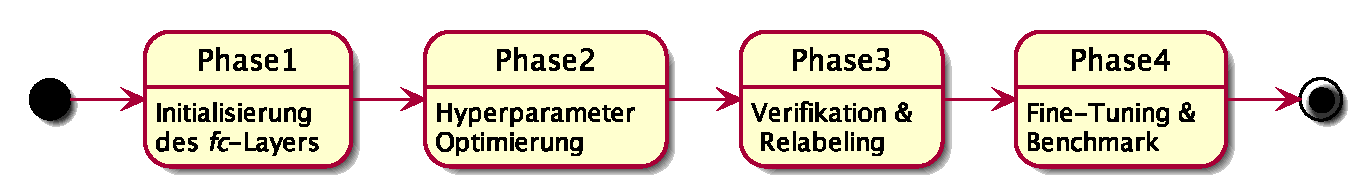
\includegraphics[width=0.9\textwidth, height=0.8\textwidth, keepaspectratio, interpolate]{fig/phases.eps}
    \caption{Ablauf der Experimente in vier Phasen}
    \label{fig:phases}
\end{figure}

Aufgrund von Hardwarebeschränkung können und sollen die Modelle nicht von Grund auf neu trainiert, sondern nur auf Basis vortrainierter Modelle nachtrainiert werden.
Kandidaten hierfür sind die Modelle SlowFast-50, ir-CSN-152 und R2+1D-34, die in der ersten Phase in Form eines einfachen Benchmarks verglichen werden.
Pro Modell findet zunächst in ein Initialisierungsschritt statt, in der (auf Basis von Kinetics) vortrainierte Gewichte in die jeweilige Modellarchitektur geladen werden.
Da die vortrainierten Modelle mit anderen Klassen und mit deutlich mehr Klassen vortrainiert wurden, wird das hinterste \fc-Layer entfernt und durch ein neues \fc-Layer mit 32 Output-Knoten für die 32 Klassen von SOCC-HAR-32 ersetzt.
Die Gewichte des neuen \fc-Layers sind im Gegensatz zu den restlichen Layern zufällig initialisiert, was ein deutliches Ungleichgewicht der Wissensverteilung innerhalb des Netzes zur Folge hat~\cite{Gugger20}.
Um die Lücke zwischen Klassifikationslayer und dem Rest des Netzes zu verringern wird in diesem Schritt ausschließlich das \fc-Layer trainiert und alle anderen Layer werden während des Trainings eingefroren.
Nach Abschluss der Initialisierung ist das Wissen deutlich gleichmäßiger verteilt und jedes der Modelle kann auf allen Layern nachtrainiert werden.
Zur Evaluation wird ein Testset mit $\Delta_\text{test}=3$ verwendet, da der maximale Zeitkontext der drei Baseline-Modelle bei 2.67 Sekunden liegt.
Basierend auf der Evaluation wird schließlich die Entscheidung für eines der drei Baseline-Modelle gefällt, welches die besten Ergebnisse liefert und in den folgenden Phasen als einziges weiter optimiert wird.
Abgeschlossen wird die Phase durch eines Verifikationsschritts und einem erneuten Training anhand der verifizierten Daten.

In der zweiten Phase werden verschiedene Konfigurationen von Hyperparametern und damit verbundenen Werte für den Zeitkontext getestet.
Da die Basiskonfigurationen aus der Literatur die untere Grenze von 3 Sekunden nicht erreichen, werden für jedes Modell die Hyperparameter $T$ und $\tau$ optimiert.
Der Zeitkontext eines Clips kann somit durch eine schnellere Abspielgeschwindigkeit (mit steigendem $\tau$) \bzw durch zusätzliche Frames (mit steigendem $T$) erhöht werden.
Einige ausgewählte Kombinationen der Hyperarameter werden im Zuge einer Grid-Suche mit vergleichsweise wenig Trainingsdaten getestet.
Die beste Konfiguration wird schließlich mit zusätzlichen Daten im größeren Umfang trainiert und anhand eines zweiten Test-Sets mit $\Delta_\text{test}=5$ evaluiert, welches auch in allen weiteren Tests genutzt wird.

In der dritten Phase werden die 32 Aktionsklassen einzeln evaluiert und Klassen, die nur extrem selten korrekt klassifiziert werden, werden aus dem ursprünglichen Datenset entfernt.
Da diese Klassen gravierenden Einfluss auf den Fehler und damit auf die Optimierung des Modells haben, wird das Netz erneut mit nur einer Untermenge der ursprünglichen Klassen nachtrainiert.
Dabei wird als weiteres Hilfsmittel Label Smoothing~\cite{Szegedy16, Mueller20} genutzt.
Anschließend folgt auch hier ein Verifikationsschritt.

In der letzten Phase werden weitere Verbesserungen der Metriken angestrebt, indem die räumliche Auflösung $S$ in Anlehnung an das Vorgehen in~\cite{Wu20} erhöht wird.

%\subsubsection*{Vergleichbarkeit mit SoccerNet}

%Das einzige veröffentlichte Datenset im Bereich Fußball ist SoccerNet.
%Daher wird schließlich mit einem speziellen Test-Set evaluiert, das genau den Testdaten von SoccerNet entspricht.
%Die beste Architektur wird mit den vortrainierten Gewichten aus Phase XL übernommen und mit SoccerNet-500 nachtrainiert und mit dem Original Testset evaluiert.
%Dieses Set weist auch die gleichen negativen Einflussfaktoren auf, wie im Original:
%\item 3) Vergleichbarkeit: Überrepräsentation von Hintergrund von X, Fehlerhafte Annotationen, Nur eine Aktion pro Spielminute


\section{Modulare Implementation}
\label{sec:konzeptuelle-umsetzung}

\begin{figure}[htbp!]
    \centering
    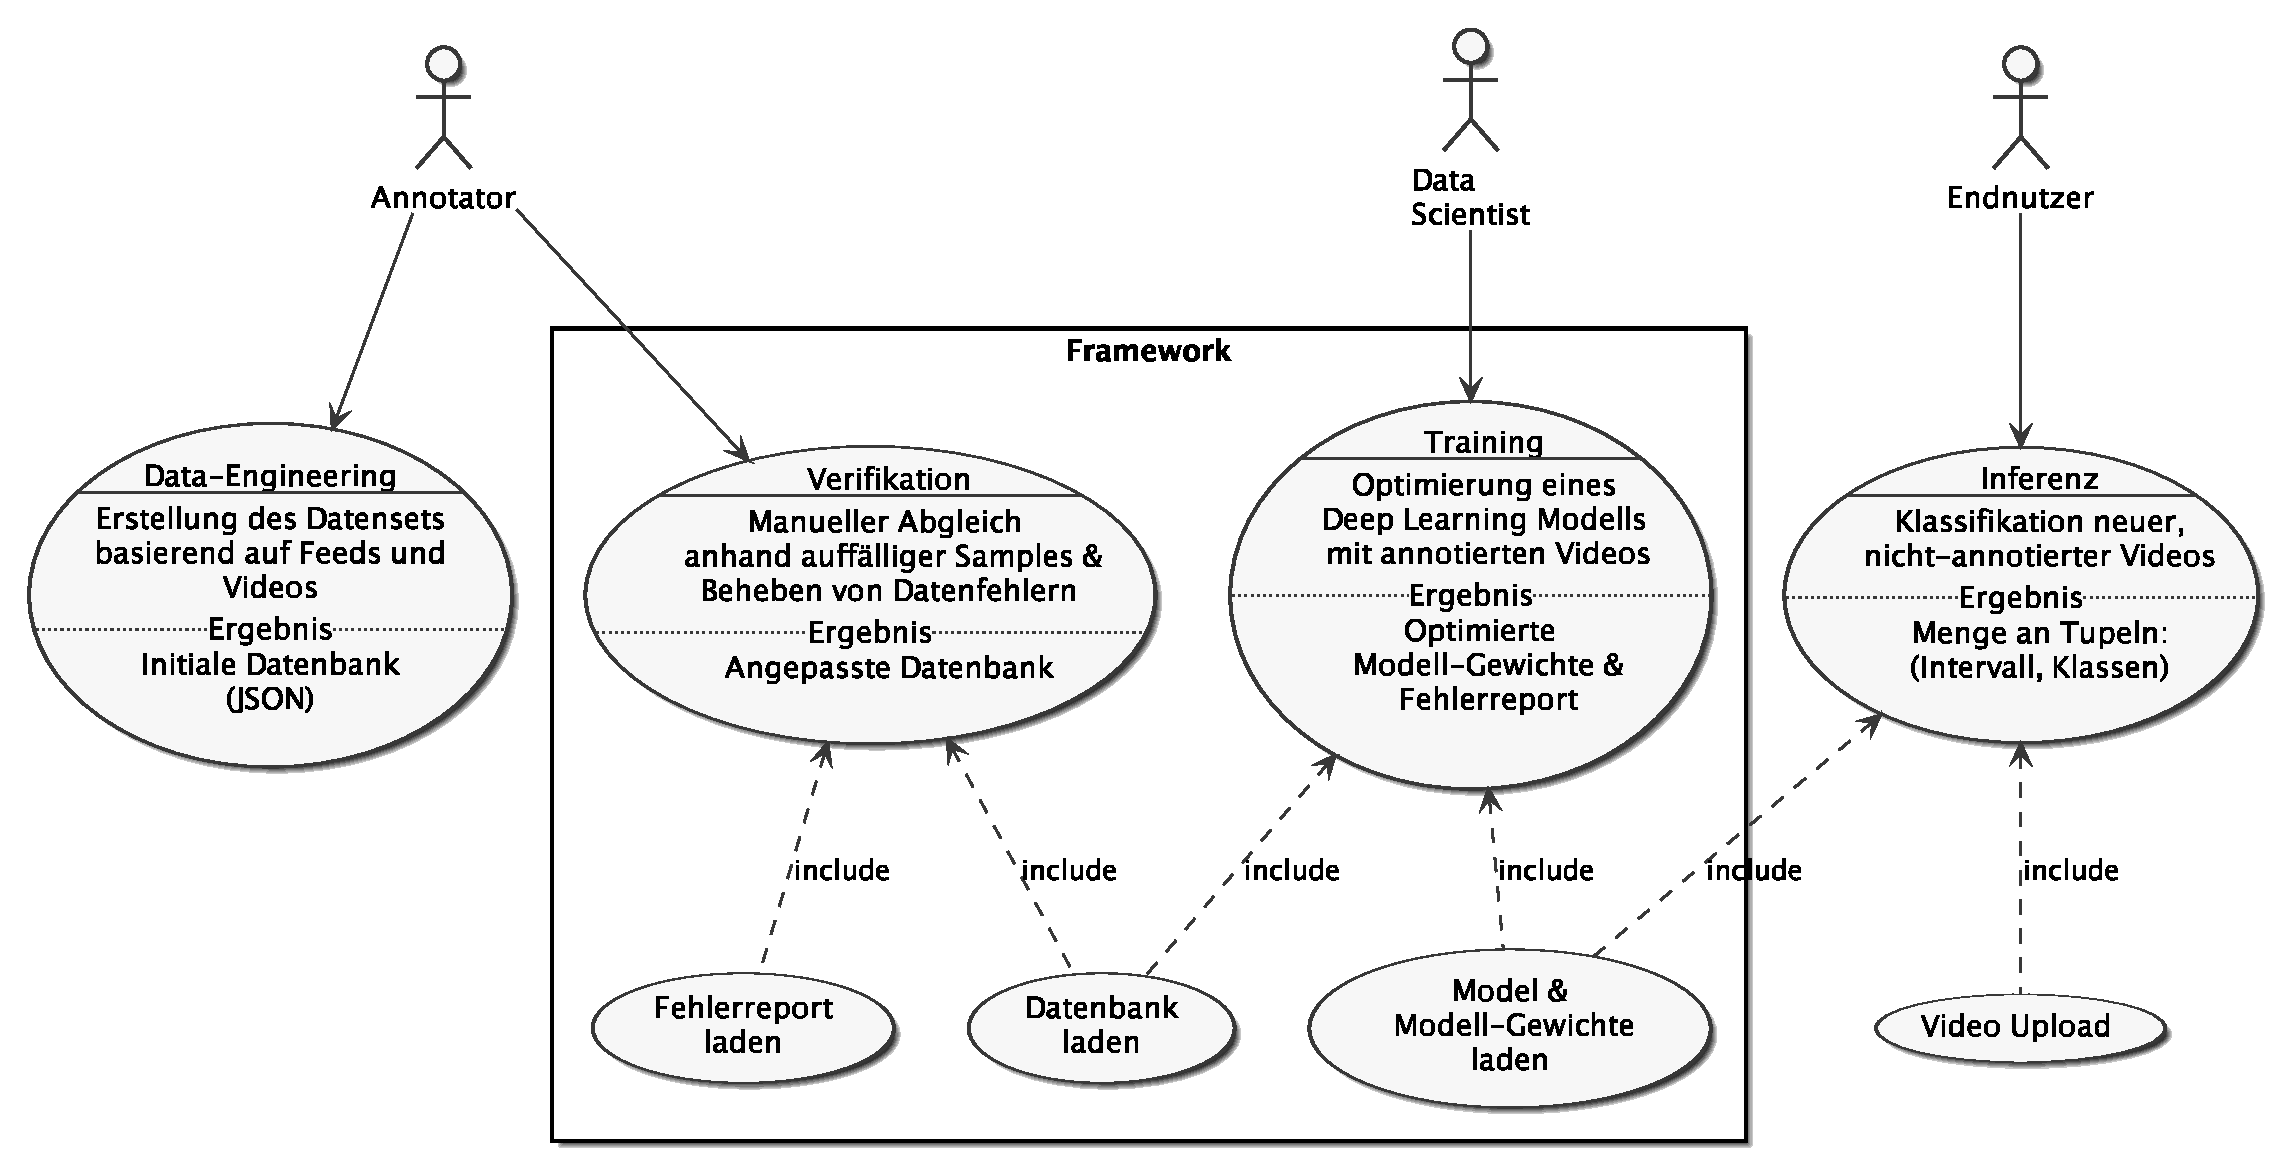
\includegraphics[width=0.9\textwidth, height=0.8\textwidth, keepaspectratio, interpolate]{fig/usecase.eps}
    \caption{Anwendungsfalldiagramm: Framework}
    \label{fig:usecase}
\end{figure}

Zur Umsetzung der Experimente wurde ein modulares Framework entwickelt, das Kernfunktionen für alle der vier, oben genannten Phasen bereitstellt und gewährleistet, dass alle Experimente einheitlich durchgeführt werden.
\autoref{fig:usecase} zeigt die Anwendungsfälle aller Zwischenschritte, beginnend mit dem Data-Engineering, das vorab einmalig ausgeführt wird und die Trainingsdaten in einer JSON-Datei speichert.
Die JSON-Datenbank bildet damit die Import-Schnittstelle zu dem Framework.

Während des Trainings die Trainingsdaten aus der Datenbank und die Modellgewichte aus entsprechenden Checkpoint-Dateien geladen.
Anhand der Trainingsdaten wird das Modell optimiert und die optimierten Gewichte werden als Ergebnis in neuen Checkpoint-Dateien persistiert.
Ebenso wird während des Trainings ein Fehlerreport erstellt, der pro Sample Metadaten, Scores und den jeweiligen Fehler der Loss-Funktion erfasst.
Dieser Report wird als weiteres Ergebnis in Form einer CSV-Datei persistiert.
Im Verifikationsschritt werden Checkpoints und Fehlerreport der potenziell besten Epoche geladen und auffällige Samples werden manuell verifiziert.
Das Ergebnis ist eine angepasste Version der initialen Datenbank, in der die erkannten Fehler behoben sind.
Der abschließende Schritt der Inferenz ist möglich mit der Export-Schnittstelle der Modellgewichte.
Das Framework schließt den vorgelagerten Zwischenschritt des Data-Engineering und den optionalen Schritt der Inferenz also nicht mit ein, stellt aber dennoch Schnittstellen für beide Prozesse zur Verfügung.

Um alle Experimente in einer generischen Umgebung durchzuführen wurde eine modulare Implementation umgesetzt, die auf den Konzepten des Frameworks Lightning \cite{Falcon19} basiert.
In \autoref{fig:modules} sind die drei Kernmodule zur Datenintegration, Training und Evaluierung schemenhaft veranschaulicht.

\begin{figure}
    \centering
    \bigimage{fig/modules-top}{0.7\textwidth}
    \caption{Module zur konzeptuellen Umsetzung}
    \label{fig:modules}
\end{figure}

Die Hyperparameter aus \autoref{subsec:hyperparameter} sind allesamt für das Datenmodul konfigurierbar.
Das Datenmodul beinhaltet Klassen zum Erstellen und Bereitstellen valider Samples, die auf Grundlage der Datenbank erzeugt und vom Training- und Evaluation-Modul in Form von Batches genutzt werden können.

Das Trainingsmodul nutzt diese Samples zur Optimierung des \gls{har}-Backbones.
Das Backbones-Modell ist dabei gegen jede andere Architektur austauschbar, sofern sie eine wohl-definierte Schnittstelle bereitstellt.
Während des Trainings werden Metriken, Checkpoint- und Fehlerreport-Dateien erfasst und an das Evaluationsmodul in Form eines Loggings übermittelt.

Das Evaluationsmodul sichert alle geloggten Daten zusammen mit weiteren Metadaten in einem Cloud-Speicher.
Auch die Hyperparameter und der Quellcode werden pro Experiment in der Cloud gesichert, sodass sich alle Ergebnisse eindeutig reproduzieren lassen.
Zudem hat das Evaluationsmodule eine Funktion zur Verifikation und kann basierend auf einem Fehlerreport die zugrunde liegende Datenbank anpassen.
